\documentclass[tikz,border=4pt]{standalone}
% bnjettag.tikzstyles.tex — TikZ preamble matching docs/style/bnjettag.mplstyle (journal pick, 2026-09-26).
% Use from a standalone figure:  % bnjettag.tikzstyles.tex — TikZ preamble matching docs/style/bnjettag.mplstyle (journal pick, 2026-09-26).
% Use from a standalone figure:  % bnjettag.tikzstyles.tex — TikZ preamble matching docs/style/bnjettag.mplstyle (journal pick, 2026-09-26).
% Use from a standalone figure:  \input{../style/bnjettag.tikzstyles.tex}
\usetikzlibrary{positioning, arrows.meta, calc, fit}
% the five precision colours, same order as the mplstyle prop_cycle
\definecolor{bnFP32}{HTML}{243746}
\definecolor{bnW8A8}{HTML}{0072B2}
\definecolor{bnW1A8}{HTML}{009E73}
\definecolor{bnW1A6}{HTML}{D55E00}
\definecolor{bnW1A4}{HTML}{CC79A7}
\definecolor{bnGate}{HTML}{990000}
\definecolor{bnStore}{HTML}{E9E9E9}
\tikzset{
  bn/.style={font=\footnotesize\rmfamily, line width=0.6pt, node distance=6mm and 6mm},
  box/.style={draw, rounded corners=1.5pt, minimum height=8mm, text width=26mm, align=center, inner sep=2pt},
  store/.style={box, fill=bnStore},
  gate/.style={box, draw=bnGate, fill=bnGate!8},
  arr/.style={-{Stealth[length=1.8mm]}},
  both/.style={{Stealth[length=1.8mm]}-{Stealth[length=1.8mm]}},
  weak/.style={arr, gray},
  data/.style={arr, font=\scriptsize\rmfamily},
}

\usetikzlibrary{positioning, arrows.meta, calc, fit}
% the five precision colours, same order as the mplstyle prop_cycle
\definecolor{bnFP32}{HTML}{243746}
\definecolor{bnW8A8}{HTML}{0072B2}
\definecolor{bnW1A8}{HTML}{009E73}
\definecolor{bnW1A6}{HTML}{D55E00}
\definecolor{bnW1A4}{HTML}{CC79A7}
\definecolor{bnGate}{HTML}{990000}
\definecolor{bnStore}{HTML}{E9E9E9}
\tikzset{
  bn/.style={font=\footnotesize\rmfamily, line width=0.6pt, node distance=6mm and 6mm},
  box/.style={draw, rounded corners=1.5pt, minimum height=8mm, text width=26mm, align=center, inner sep=2pt},
  store/.style={box, fill=bnStore},
  gate/.style={box, draw=bnGate, fill=bnGate!8},
  arr/.style={-{Stealth[length=1.8mm]}},
  both/.style={{Stealth[length=1.8mm]}-{Stealth[length=1.8mm]}},
  weak/.style={arr, gray},
  data/.style={arr, font=\scriptsize\rmfamily},
}

\usetikzlibrary{positioning, arrows.meta, calc, fit}
% the five precision colours, same order as the mplstyle prop_cycle
\definecolor{bnFP32}{HTML}{243746}
\definecolor{bnW8A8}{HTML}{0072B2}
\definecolor{bnW1A8}{HTML}{009E73}
\definecolor{bnW1A6}{HTML}{D55E00}
\definecolor{bnW1A4}{HTML}{CC79A7}
\definecolor{bnGate}{HTML}{990000}
\definecolor{bnStore}{HTML}{E9E9E9}
\tikzset{
  bn/.style={font=\footnotesize\rmfamily, line width=0.6pt, node distance=6mm and 6mm},
  box/.style={draw, rounded corners=1.5pt, minimum height=8mm, text width=26mm, align=center, inner sep=2pt},
  store/.style={box, fill=bnStore},
  gate/.style={box, draw=bnGate, fill=bnGate!8},
  arr/.style={-{Stealth[length=1.8mm]}},
  both/.style={{Stealth[length=1.8mm]}-{Stealth[length=1.8mm]}},
  weak/.style={arr, gray},
  data/.style={arr, font=\scriptsize\rmfamily},
}

\begin{document}
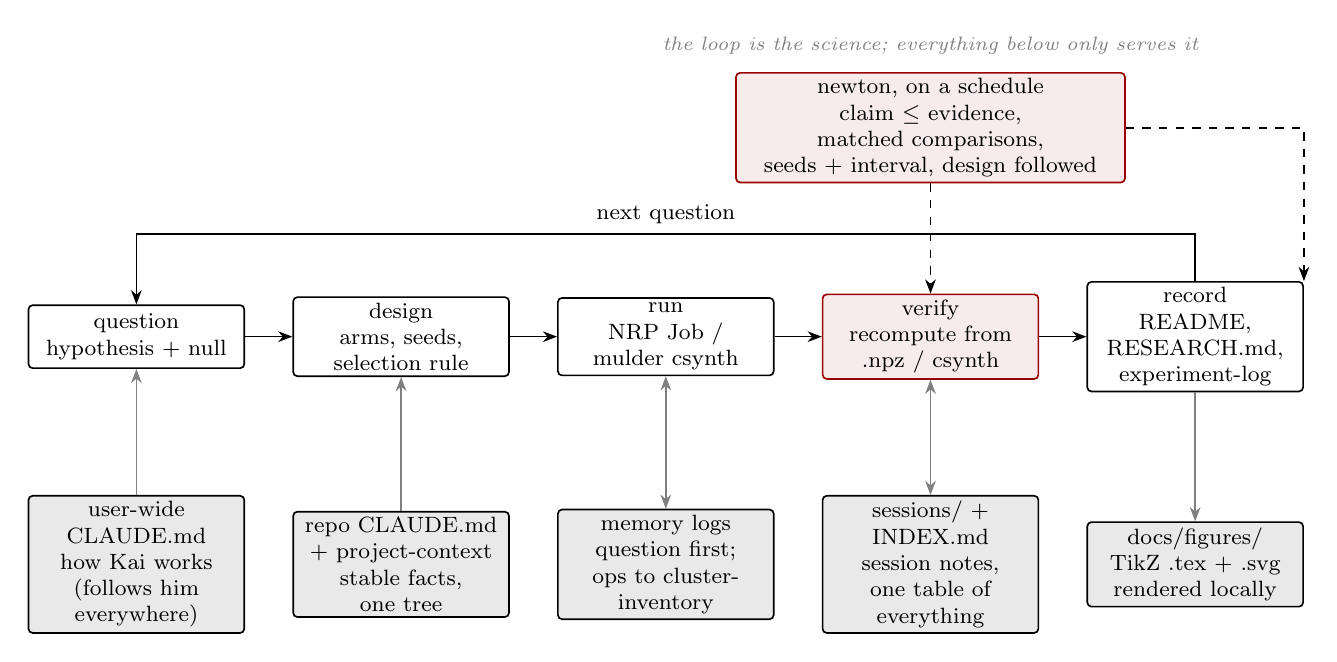
\begin{tikzpicture}[
  bn,
]
\node[box] (q) {question\\hypothesis + null};
\node[box, right=of q] (d) {design\\arms, seeds,\\selection rule};
\node[box, right=of d] (run) {run\\NRP Job /\\mulder csynth};
\node[gate, right=of run] (v) {verify\\recompute from\\.npz / csynth};
\node[box, right=of v] (rec) {record\\README,\\RESEARCH.md,\\experiment-log};
\draw[arr] (q) -- (d);
\draw[arr] (d) -- (run);
\draw[arr] (run) -- (v);
\draw[arr] (v) -- (rec);
\draw[arr] (rec.north) -- ++(0,6mm) -| (q.north) node[pos=0.25, above] {next question};

\node[gate, text width=48mm, above=14mm of v] (newton) {newton, on a schedule\\claim $\le$ evidence, matched comparisons,\\seeds + interval, design followed};
\draw[arr, dashed] (newton.south) -- (v.north);
\draw[arr, dashed] (newton.east) -| (rec.north east);

\node[store, below=16mm of q] (prefs) {user-wide CLAUDE.md\\how Kai works\\(follows him everywhere)};
\node[store, right=of prefs] (facts) {repo CLAUDE.md\\+ project-context\\stable facts, one tree};
\node[store, right=of facts] (logs) {memory logs\\question first;\\ops to cluster-inventory};
\node[store, right=of logs] (vault) {sessions/ + INDEX.md\\session notes,\\one table of everything};
\node[store, right=of vault] (figs) {docs/figures/\\TikZ .tex + .svg\\rendered locally};

\draw[arr, gray] (prefs.north) -- (q.south);
\draw[arr, gray] (facts.north) -- (d.south);
\draw[both, gray] (logs.north) -- (run.south);
\draw[both, gray] (vault.north) -- (v.south);
\draw[arr, gray] (rec.south) -- (figs.north);

\node[above=1mm of newton, font=\scriptsize\rmfamily\itshape, gray, text width=70mm, align=center] {the loop is the science; everything below only serves it};
\end{tikzpicture}
\end{document}
